\documentclass[twocolumn]{article}
\usepackage[a4paper, top=1in, bottom=1in, left=2cm, right=2cm]{geometry}
\usepackage[onehalfspacing]{setspace}
\usepackage{amsmath}
\usepackage{amssymb}
\usepackage{graphicx}
\usepackage{kotex}
\usepackage{hyperref}
\title{평면 경계면에 의한 굴절 상과 아스트로이드의 재발견}
\author{M. Ryu \\ {\href{mailto:mingshey@hafs.hs.kr}{mingshey@hafs.hs.kr}}}
\begin{document}
\maketitle
\section{도입}
물에 담긴 연필이 꺾여 보이는 현상은 빛의 굴절을 배울 때 가장 먼저 접하는 친숙한 광경이다. 
하지만, 유심히 관찰해 보면 연필 끝이 항상 같은 위치에 있는 것처럼 보이지 않는다는 사실을 
알 수 있다. 정확히 위에서 내려다볼 때의 겉보기 깊이는 일반물리학 시간에 다루지만, 비스듬히 볼 
때의 깊이 및 수평 위치는 얼마만큼 다르게 보이는가? 아마도 그다지 중요하지 않거나, 중요도에
비해 너무 복잡하여 깊이 다루지 않는 것이라 생각할 수 있다. 실제로 고급 광학 교재에서도 
렌즈나 거울과 같은 더욱 중요한 주제에 가려져 이 간단한 질문은 쉽게 잊히곤 한다.

하지만 이처럼 단순해 보이지만 흥미로운 질문은 때때로 우리의 호기심을 자극한다. 필자뿐만 
아니라 이 질문에 대한 답을 궁금해하는 사람들이 있을 것이다. 이 글에서는 이에 대한 해답을 
제시하고자 한다.

\section{간단한 해답}

\hfill 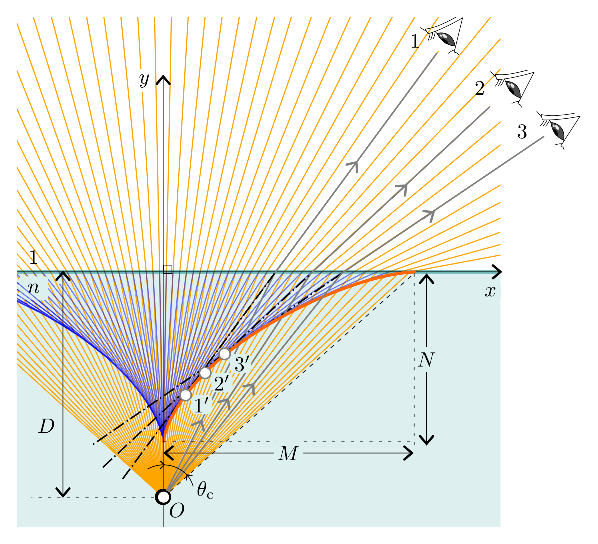
\includegraphics[width=2.7in]{g409.eps} \hfill\null

호기심은 있지만 시간을 많이 할애하기 어려운 독자를 위해 결론부터 말하자면 이렇다:  
평평한 수면 아래의 점 물체를 수면 위에서 바라볼 때, 상의 위치는 시점(POV)에 따라 달라진다. 
시점이 움직임에 따라 법평면 내에서 관찰되는 상의 자취는 일종의  코스틱\footnote{허상의 
자취이므로 ``허코스틱''(\emph{virtual caustic}) 이라고 할 수 있겠다.}인데, 이 경우에 
코스틱은 ``찌그러진 아스트로이드''라고 불리는 특정 곡선이다.
	
물체와 시점을 포함하는 법평면을 $xy$-평면으로 하고, 법평면과 수면의 교선을 $x$-축으로, 
물체를 통과하는 법선을 $y$-축으로 하자. 그러면 상의 자취는 다음 곡선의 일부이다.
	$$ \left| \dfrac{x}{M} \right| ^ {2/3} 
	+ \left| \dfrac{y}{N} \right| ^ {2/3} = 1,$$
여기서 $M = D/\sqrt{n^2 - 1}$은 전반사의 임계각에 의해 결정되는 입사 거리의 최댓값이고, 
$N = D/n$은 바로 위에서 관찰할 때 물체의 겉보기 깊이이며, 
$D$는 물체의 실제 깊이이고, $n$은 공기에 대한 물의 굴절률이다.
	
\section{공식의 유도}
	
공기와 물의 굴절률을 각각 $n_1$ 및 $n_2$라고 하자. 공기와 물의 경계면 아래 깊이 $D$인 곳에 점 물체 $O$가 있다. 
물체에서 출발한 광선이 $y$-축으로부터 $\alpha$만큼 떨어진 경계면 위의 점 A에 
법선으로부터 $\theta_2$의 각도로 입사한 후, 동일한 법선으로부터 $\theta_1$의 각도로 공기 중으로 굴절된다.

\hfill 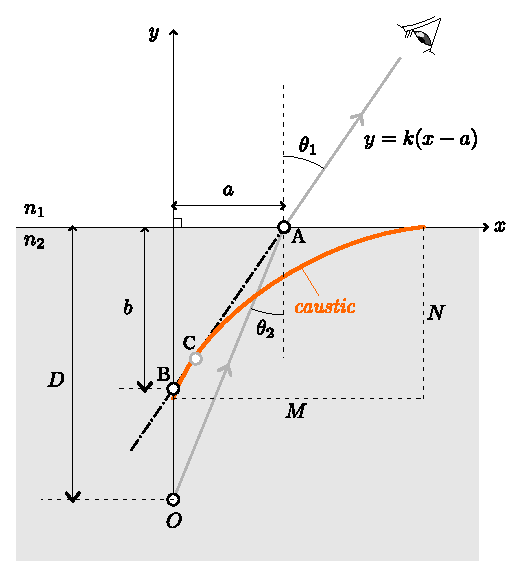
\includegraphics[width=2.2in]{g237.eps}\hfill\null\\

이 때 스넬의 법칙에 따라 다음이 성립한다.
$$ \sin\theta_1 = \frac{n_2}{n_1} \sin\theta_2 = n\sin\theta_2.$$
굴절된 광선의 연장선은 다음 방정식으로 표현된다.
$$y=k(x-\alpha).$$
여기서 
$$k=\dfrac{1}{\tan\theta_1}=\dfrac{\cos\theta_1}{\sin\theta_1}$$
이고, 스넬의 법칙을 고려하면,
$$k=\dfrac{\sqrt{1-n^2\sin^2\theta_2}}{n\sin\theta_2}.$$
이 직선은 $y$-축과 점 B($y=\beta$)에서 만나므로,
$$\beta = -k\alpha.$$
기하학적으로 다음을 얻을 수 있다.
$$\alpha = D\tan\theta_2 = \dfrac{D\sin\theta_2}{\cos\theta_2},$$
및
$$\begin{aligned}
	\beta &= -k\alpha \\
	&= -\dfrac{D\sin\theta_2}{\cos\theta_2}
	\dfrac{\sqrt{1-n^2\sin^2\theta_2}}{n\sin\theta_2}\\
	&=-\dfrac{D\sqrt{1-n^2\sin^2\theta_2}}{n\cos\theta_2}.
\end{aligned}$$
이제, $K=\alpha/M$ 및 $H=\beta/N$이라 하면,
$$ \begin{aligned}
	K^2 + H^2 &= \dfrac{\alpha^2}{M^2}+\dfrac{\beta^2}{N^2}\\
	&=\dfrac{\left(n^2-1\right)\sin^2\theta_2 + 1-n^2\sin^2\theta_2}
	{\cos^2\theta_2}\\
	&=\dfrac{1-\sin^2\theta_2}{\cos^2\theta_2}\\
	&=1
\end{aligned}$$
$\xi=x/M$ 및 $\eta=y/N$이라고 하면, 시점이 $xy$-평면에서 움직임에 따라,
점 $\mathrm{A}(\alpha, 0)$ 및 $\mathrm{B}(0, \beta)$도 이에 따라 움직이는데, 
점  $\mathrm{A}$, $\mathrm{B}$는 각각  $\xi\eta$-평면의 점 $\mathrm{K}(K, 0)$
및 $\mathrm{H}(0, H)$에 대응된다. 이 때 두 점 $\mathrm{K}$, $\mathrm{H}$ 사이의 
거리는 $1$로 일정하게 유지된다.

선분 $\overline{\mathrm{KH}}$의 포락선은 `아스트로이드'(%
\href{https://en.wikipedia.org/wiki/Astroid}{\emph{astroid}}\footnote{
소행성을 뜻하는 \emph{asteroid}와 혼동하지 말 것.})로 잘 알려져 있으며, 
다음 방정식으로 표현된다.
$$ \left| \xi \right|^{2/3} + \left| \eta \right|^{2/3} = 1. $$

\hfill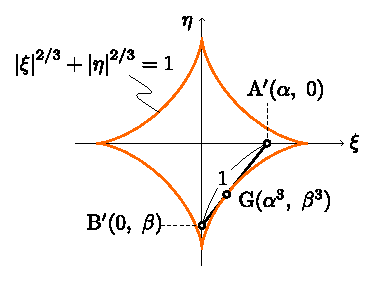
\includegraphics{g107.eps} \hfill\null

상은 선분 $\overline{\mathrm{AB}}$와 포락선의 접점 $\mathrm{C}$에 위치한다. 
이는 이 순간 인접한 광선 다발이 발산하는 점이기 때문이다. 
$\xi\eta$-평면에서 해당 점은 $\mathrm{G}(K^3, H^3)$이다.
	
따라서 다음 관계식으로부터 상의 좌표 $(x_{\mathrm{C}}^{}, y_{\mathrm{C}}^{})$를 얻을 수 있다.
$$ \left\{ 
\begin{aligned}
	\xi_{\mathrm{C}}^{} &= \dfrac{x_{\mathrm{C}}^{}}{M} = K^3 = \dfrac{\alpha^3}{M^3},\\
	\eta_{\mathrm{C}}^{} &= \dfrac{y_{\mathrm{C}}^{}}{N} = H^3 = \dfrac{\beta^3}{N^3}.
\end{aligned}
\right.$$
즉,
$$ \left\{ 
\begin{aligned}
	x_{\mathrm{C}}^{} &= \dfrac{\alpha^3}{M^2},\\
	y_{\mathrm{C}}^{} &= \dfrac{\beta^3}{N^2}=-\dfrac{k^3\alpha^3}{N^2}.
\end{aligned}
\right.$$

여기서
	$$\sin\theta_2 = \dfrac{\alpha}{\sqrt{D^2+\alpha^2}}$$
를 이용하여
$$k = \dfrac{\sqrt{D^2-(n^2-1)\alpha^2}}{n\alpha},$$
를 얻을 수 있으며, 
상의 위치를 $\alpha$에 대한 매개변수 함수로 유도할 수 있다.
$$ \left\{ 
\begin{aligned}
	x_{\mathrm{C}}^{} &= (n^2-1)\dfrac{\alpha^3}{D^2},\\
	y_{\mathrm{C}}^{} &= -\dfrac{n^2}{D^2}\dfrac{\alpha^3}
	{n^3\alpha^3}\left\{ D^2-(n^2-1)\alpha^2 \right\}^{3/2}\\
	&=-\dfrac{D}{n}\left\{ 1-(n^2-1)\dfrac{\alpha^2}{D^2} \right\}^{3/2}.
\end{aligned}
\right.$$
	
\section{시점이 물 속에 있는 경우}

물체가 경계면 위 높이 D인 공기 중에 있고, 
시점이 물 속에 있는 경우, 상대적인 굴절률은 $1/n < 1$이고, 
유사한 추론에 의해 코스틱에 대한 다음 방정식을 얻는다.
$$ \left| \xi \right|^{2/3} - \left| \eta \right|^{2/3} = -1, $$
여기서 $\xi = \dfrac{x}{W} $ 및 $\eta = \dfrac{y}{Z}$이고, 
$W = \dfrac{nD}{\sqrt{n^2-1}}$ 및 $Z = nD$인데,  이 곡선은 기울기가 
$\pm Z/W = \pm \sqrt{n^2-1}$인 점근선을 갖는다.

따라서 물 속에서 본 물 위 하늘의 풍경은
연직선으로부터 전반사의 임계각 안쪽 원(또는 원뿔) 안에 압축되어 보인다. 이것은 
`스넬의 창'(Snell's window)이라고 하는 잘 알려진 현상이며 전천 사진과 같은 초광각 
사진에 사용되는 어안렌즈(fisheye lens)의 시야와도 닮았다.

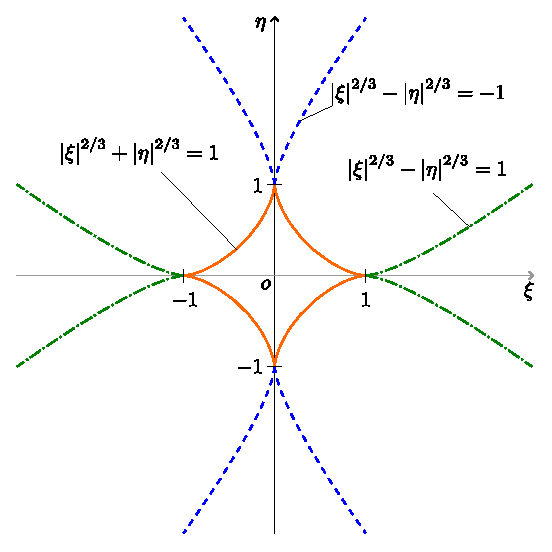
\includegraphics[width=3in]{g254.eps}

이 곡선의 좀 더 일반적인 형태인 
$$ \left| \xi \right|^{2/3} - \left| \eta \right|^{2/3} = \pm1 $$
은 물리학적으로 물 위의 점광원에서 나와 물 속으로 들어가며 굴절된 광선들의 코스틱 
곡선으로 등장하기도 하는데, 필자가 아는 바로는 아직 이름이 확립되지 않은 것같다.
여기에 `쌍곡-아스트로이드'(\emph{hyperastroid})라고 이름을 붙여보는 것은 어떨까?
아스트로이드에 대해 이 곡선은 타원에 대한 쌍곡선과도 비슷한 관계가 있기 때문이다. 
 
아스트로이드는 
$$ \left| \xi \right|^{r} + \left| \eta \right|^{r} = 1. $$
와 같이 정의되는 `초타원'(\href{https://mathworld.wolfram.com/Astroid.html}%
{\emph{superellipse}})이라는 곡선 계열에 속한다. 
아스트로이드는 $r=2/3$인 경우이다.
 
그러나 필자가 알기로는 다음 형태의 곡선 계열에 대한 이름도 없다.
$$ \left| \xi \right|^{r} - \left| \eta \right|^{r} = \pm 1 $$
이것은 `초쌍곡선'(\emph{super-hyperbola}\footnote{같은 의미의 반복되는 어원
때문에 거슬릴 수도 있으니 \emph{superbola}라고 하는 것이 
좋을 수도 있겠다.})이라고 부를 수 있을지 모르겠다.

\section{상의 위치 찾기}
물체에 대한 허상의 코스틱을 닫힌 형태로 구할 수 있으므로 이를 이용하여 물체의 위치와 
시점이 주어졌을 때 상의 위치를 다음과 같이 찾을 수 있다.

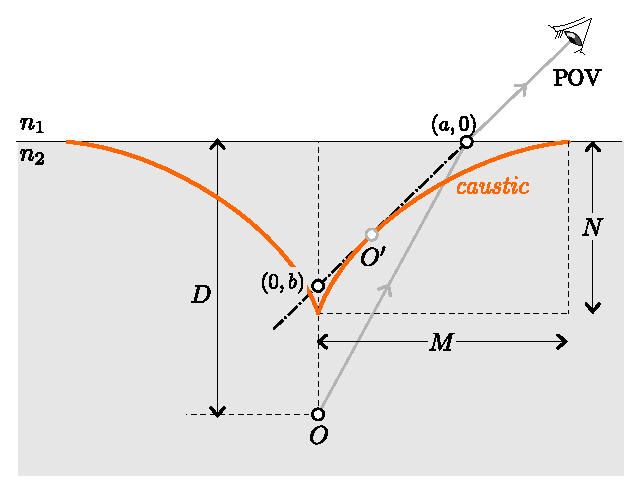
\includegraphics[width=3in]{g394.eps}

시점에서 코스틱에 접선을 그린다. 접선과 코스틱의 접점이 상의 위치이고, 접선이 수면과 
교차하는 점은 물체에서 나온 광선이 수면에 입사하는 점이다.

물 속에 연속된 물체가 있다면 물체의 표면을 따라 놓인 점 $1, 2, 3, \dots$ 에 대해 
각각 이와 같은 방법으로 상을 찾을 수 있다. 점이 연속으로 움직일 때 따라 움직이는 상의 자취가 
물체의 상이 될 것이다.

\includegraphics*[width=3in]{g240.eps}

단, 코스틱에 대한 접선은 해석적으로 찾기 어렵고 실제로는 수치적인 방법을 이용하여 
근삿값을 찾는 것으로 만족해야 할 것이다.

또다른 방법은 물체와 시점을 잇는 광선의 경로를 페르마의 원리를 이용하여 수치적으로 
구한 다음, 광선이 수면과 교차하는 점의 좌표를 바탕으로 아스트로이드의 접점 공식을 이용하여
상의 위치를 구하는 방법이다. 이에 대한 파이썬 예제는  
\href{https://github.com/mingshey/python_projects/blob/main/Refraction_Image.ipynb}%
{github.com/mingshey/python\_projects} 에 있다.


\appendix
\section*{부록: 포락선으로 정의한 아스트로이드}
평면 상의 직교 좌표에서 $x$ 축 위의 점  $(K, 0)$과 $y$ 축 위의 점 $(0, H)$가 일정한 거리 $a$를 유지하며 움직인다고 하자. 그러면 $K^2+H^2=a^2$이고, 어느 순간 선분을 포함하는 직선의 방정식을 
$$y=-\dfrac{H}{K}(x-K)$$
라 쓸 수 있고, $H=\pm \sqrt{a^2-K^2}$임을 이용하면 
$$y(x, K) = \mp \dfrac{\sqrt{a^2-K^2}}{K}(x-K)$$
라 할 수 있다. 
$K$값이 변할 때 두 점을 잇는 선분 또는 직선이 변하며 그리는 포락선은 매 순간 정류점들의 자취, 즉
\newcommand{\pardiff}[2]{{\frac{\partial #1}{\partial #2}}}
\newcommand{\ilpardiff}[2]{{{\partial #1}/{\partial #2}}}
$\ilpardiff{y}{K} = 0$인 점들의 자취이다. 이 조건을 만족하는 $(x, y)$들을 구해 보자.

$$ \begin{aligned}
\pardiff{y}{K} &= \pm\left[\left( \dfrac{1}{\sqrt{a^2-K^2}}+\dfrac{\sqrt{a^2-K^2}}{K^2}\right) (x-K) + \dfrac{\sqrt{a^2-K^2}}{K} \right]\\
	&= \pm \dfrac{(K^2+a^2-K^2)(x-K)+K(a^2-K^2)}{K^2\sqrt{a^2-K^2}}\\
	&= \pm \dfrac{a^2 x - K^3}{K^2 \sqrt{a^2 - K^2}}\\
	&= 0.
\end{aligned}
$$
따라서 정류점의 $x$좌표는 $x = K^3/a^2$ 이고, 이 때 $y$좌표의 값은

$$ \begin{aligned}
y(x, K) &= \mp \dfrac{\sqrt{a^2-K^2}}{K}\left(\dfrac{K^3}{a^2}-K\right)\\
	& = \pm \dfrac{\left( a^2- K^2 \right)^{3/2}}{a^2}\\
	& = \dfrac{H^3}{a^2}
\end{aligned}
$$
이다. 따라서 정류점의 좌표 $(x, y)$는 다음 방정식을 만족한다:
$$ \left|\dfrac{x}{a}\right|^{2/3} + \left|\dfrac{y}{a}\right|^{2/3} = 1. $$
$\blacksquare$

\end{document}